\subsection{Strip Tracker Calibrations}

The CMS SiStrip detector plays a critical role in the High-Level Trigger (HLT) decision-making process. The calibration of its parameters, particularly for tracking and reconstruction, is vital for maintaining performance and ensuring robust data acquisition. This document summarizes the key prospects and current practices for optimizing SiStrip calibrations at HLT.\\
Out of the 326 conditions in the HLT GT, 24 are related to the Silicon Strip Tracker, of which 21 are relevant to Run 3 data-taking. From these, the following 4 are considered core and critical for data-taking:

\begin{table}[h!]
    \centering
    \begin{adjustbox}{max width=\textwidth}
    \begin{tabular}{p{3.5cm}|p{4cm}|p{2.5cm}|p{2cm}|p{4.5cm}}
        \textbf{Name} & \textbf{Record} & \textbf{Workflow} & \textbf{Frequency of Updates} & \textbf{Description} \\ \hline
    \end{tabular}
    \end{adjustbox}
    \caption{Fundamental SiStrip Calibrations, ordered in terms of frequency of updates.}
    \label{tab:StripCalibrations_critical}
\end{table}

\subsubsection{DAQ O2O conditions}
 The Strip DAQ O2O populates tracker conditions from the online master data storage (OMDS) to the offline reconstruction conditions database (ORCON). 
Six types of payloads are populated in this O2O: 
\begin{itemize}
\item \texttt{SiStripBadStrip} 	
\item \texttt{SiStripFedCabling} 	
\item \texttt{SiStripLatency} 	
\item \texttt{SiStripNoises} 	
\item \texttt{SiStripPedestals} 	
\item \texttt{SiStripThreshold}
\end{itemize}

\subsubsection{DCS O2O conditions}
 The Strip DCS O2O populates tracker HV/LV information from PVSS database to the offline condition database (\texttt{ORCON}). This DCS info is used in prompt reconstruction. Modules that are OFF are retrieved form the PVSS database and stored in the condition database via hourly cron jobs. Three cron jobs are set up for the DCS O2O, including one production job and two validation jobs, each write to a different tag in the condition database with a different delay in time: 
\begin{itemize}
\item 1 hour Delay Validation: populates HV/LV states until 1 hour before the cron job execution;
\item 13 hours Delay Validation: populates HV/LV states until 13 hour before the cron job execution;
\item 25 hourse Delay Validation: populates HV/LV states until 25 hours before the cron job execution. Also synchronized to the tag used in production for prompt reco;
\end{itemize}

\subsubsection{Bad Components}

For the identification of bad components dedicated to a given run it is important that the analysis is based on data which do not take into account the knowledge of bad components identified during the offline analysis of previous runs. This has to be ensured because bad components might be recovered from one run to another so that they have to be qualified unbiased afterwards. Since the reconstruction chain used to produce the usual tracker AlCaReco streams already includes bad components from offline analysis, these streams cannot be used here.

Therefore, a \texttt{AlCaReco} stream dedicated to the bad component identification in the strip tracker was introduced in the \texttt{AlCaReco} workflow. It is called \texttt{ALCARECOSiStripCalZeroBias} and has the following properties:
\begin{itemize}
\item  The input are the digis from standard reconstruction since they are independent from bad channel masking. The reconstruction is performed up to cluster (so only the digi to cluster step is performed in the AlCaReco).
\item Only bad components from cabling and o2o are taken into account during reconstruction. Bad components from offline analysis are not considered.
\item Only events with random trigger are selected. For collision data the HLT path \texttt{HLT\_ZeroBias} and for cosmic data the \texttt{HLT\_Random} is chosen.
\item The output of the stream contains only the cluster collection and the \texttt{L1AcceptBunchCrossings} collection (needed by the filters against APV induced noise). This can be used as starting point in case the calibration has to be redone.
\item The DQM output contains one cluster occupancy histogram per strip detector. These histograms are used as input for the bad component algorithms. In addition, the \texttt{ClusterVsAPVCycle} and the \texttt{TotalNumberOfCluster} histograms are stored for each subdetector. 
\end{itemize}

Once the DQM output of a given run with enough statistics is available from the central DQM harvesting, the bad component identification can be performed.

\begin{figure}[htbp]
   \centering
	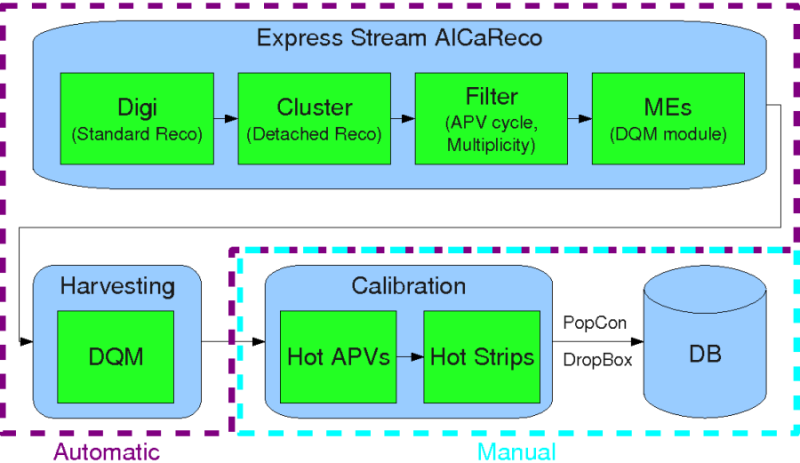
\includegraphics[width=0.7\textwidth]{figures/BadComponentWorkflow_small.png}
   \caption{The workflow for the Bad Component Identification is shown in the sketch above.}
   \label{fig:fill10200PCL}
\end{figure}

\subsubsection{APV gains}
The gain calibration is performed in two sequential steps, each one delivering a
calibration factor. These steps, referred as the calibration sequence, are:

\begin{itemize}
\item Tick Mark calibration (\texttt{SiStripApvGainRcd}): the tick marks are external signals, input into the readout chips every 35 LHC clocks, that are used to synchronize the tracker modules to the central trigger.
When the detector is synchronized, the height of the voltage pulse at the tick mark is equalized in gain among all the readout chips to 640 ADC counts. This calibration corrects for the electronic effects at the readout level but does not account for the differences at the sensor level.\\
This is performed via the so-called tickmark O2O 
\item Particle Calibration (\texttt{SiStripApvGain2Rcd}): the particle calibration equalizes the detector response for the measurement of the m.i.p. charge. \\
The charge measured by each cluster on track is corrected for the track path in the sensor depletion region and therefore used to build the distribution of the ionization charge per unit of length. The voltage gain is tuned to have the most probable value of these distributions, made for every sensors, set to 300 ADC counts / mm. This procedure requires a lot of track statistics (around 1B clusters).\\
This is performed via a multi-run harvesting based PCL workflow.
\end{itemize}

\subsubsection{CPE conditions}

\begin{itemize}
    \item Two key CPE-related conditions are maintained:\newline
    \texttt{SiStripLorentzAngleRcd} and \texttt{SiStripBackPlaneCorrectionRcd}.
    \item Both conditions are provided in two configurations: "deconvolution" and "peak," depending on the readout mode.
    \item Updates to these calibrations require dedicated workflows involving special datasets (e.g., cosmics, low pile-up collisions).
    \item The conditions have seen minimal updates since early Run 2, as miscalibrations are often treated as geometric mispositioning during tracker alignment procedures.
    \item A monitoring workflow exists in the Prompt Calibration Loop (PCL), but direct calibration at HLT is limited.
\end{itemize}

\subsubsection*{Future Prospects and Integration in NGT Demonstrator Workflow}
\begin{itemize}
    \item \textbf{Bad Components Masking}:
    \begin{itemize}
        \item Already implemented in PCL workflows and requires minimal statistics for updates.
        \item Demonstrated to improve track building in inside-out muon reconstruction.
    \end{itemize}
    \item \textbf{G2 Gains Calibration}:
    \begin{itemize}
        \item High-statistics requirement makes frequent updates infeasible.
        \item Potential minor impact on track building and cluster charge thresholds.
    \end{itemize}
\end{itemize}

\subsubsection*{Recommendations}
\begin{itemize}
    \item Prioritize the inclusion of bad components masking in the NGT demonstrator workflow due to its operational simplicity and demonstrated impact.
    \item Consider periodic evaluations for integrating gain calibrations as part of long-term upgrades.
\end{itemize}